% !TEX root = ../intro-stellar-physics.tex

We saw in chapter~\ref{ch.basic-stellar-properties} that the equilibrium central temperature of a self-gravitating object---such as a star---with an ideal gas EOS depends \emph{solely} on the mass, radius, and composition of that star. For the sun, this temperature is $\approx \val{15}{\Mega\K}$ and is much higher than the surface effective temperature $T_{\!\mathrm{eff,\odot}} = \val{5780}{\K}$. We don't see X-rays coming from the interior of the sun; the photons emitted from the sun are all coming just from the cooler surface layers.

\newthought{Photons in a plasma, such as in the interior of the sun, transport energy.}  Were the sun transparent, these photons would immediately stream out, and the sun would release its stored energy in a fiery blast.  This doesn't happen: a photon can only travel a short distance before being scattered or absorbed. The net effect is that photons generated in the core must travel a tortuous path, rather like a pinball, before reaching the surface and escaping.

\section{Interaction of radiation and matter}\label{s.interaction-radiation-matter}

How far does a photon---or any particle, for that matter---travel, on average, in the interior of the sun? Imagine a particle traveling with speed $v$.  Draw a cylinder, of length $\ell$ and cross-sectional area $\mathcal{A}$, around its path, as shown in Fig.~\ref{f.MFP}. What the particle ``sees'' is that the cylinder is partly blocked by obstacles---other particles in its path.
\begin{marginfigure}
    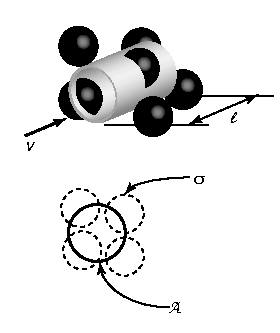
\includegraphics[width=\linewidth]{mean-free-path}
    \caption[Schematic of mean free path]{\label{f.MFP} Schematic of a particle incident on a group of scattering or absorbing particles.}
\end{marginfigure}
What is the probability of our particle making it through the cylinder unscathed? The probability of the particle hitting an obstacle is the ratio
\[
    \mathcal{P} = \frac{\textrm{total area covered by obstacles}}{\textrm{area of cylinder}}
\]
Denote the cross-sectional area of each particle by $\sigma$. If the density of particles is $n$, then the number of obstacles in the cylinder is $n\times(\mathcal{A}\ell)$, and therefore the fraction of the area blocked by the obstacles is
\marginnote{We are taking $\ell$ and $\mathcal{A}$ sufficiently small that we don't have to worry about particles overlapping.}
\begin{equation}
    \mathcal{P} = \frac{n\times(\mathcal{A}\ell)\times\sigma}{\mathcal{A}} = n\sigma\ell.
\label{e.prob-MFP}
\end{equation}
The particle will suffer a collision when $\mathcal{P}\to 1$, or when
\begin{equation}\label{e.MFP}
    \ell = \frac{1}{n\sigma}.
\end{equation}
We call $\ell$ the ``mean free path'': it is the mean distance the particle travels freely before colliding.

\begin{marginfigure}[3\baselineskip]
    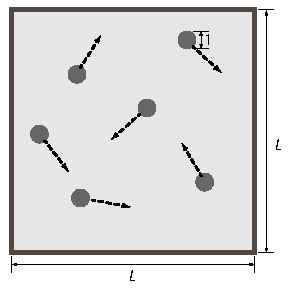
\includegraphics[width=\linewidth]{air-hockey-mfp}
    \caption[Mean free path of a hockey puck]{\label{f.MFP-2D}Schematic for Exercise~\ref{ex.MFP-2D}}
\end{marginfigure}
\begin{exercisebox}[Mean free path of a hockey puck]\label{ex.MFP-2D}
    Suppose we have a flat, slippery surface on which hockey pucks are sliding around, as shown in Fig.~\ref{f.MFP-2D}. The pucks bounce off the walls as they slide around.  Suppose there are $N$ pucks, each with unit diameter, and the table is square with sides of length $L$.  Estimate the mean free path of a puck.
\end{exercisebox}

Although we have motivated this derivation with a classical picture, since the cross-section $\sigma$ is just related to the probability of an interaction we can define it for quantum mechanical systems as well.

\begin{exercisebox}[Mean free path for electron scattering]\label{ex.MFP}
    In the sun, free electrons scatter photons; the cross-section for this is
    \[
    \sigma_{\mathrm{Th}} = \left(\frac{8\pi}{3}\right)\left(\frac{e^2}{4\pi\epsilon_{0}\,m_e c^2}\right)^2 = \val{\sci{6.65}{-29}}{\meter^2}.
    \]
    What is the mean free path against this process for a photon at the average density of the solar interior?
\end{exercisebox}

As the ray of light traverses a small distance $\Delta s$ through some matter, the probability of a photon being absorbed is $\mathcal{P} = n\sigma\Delta s$. Thus, out of every $N$ photons, $\Delta N = N \times\mathcal{P} = N\times n\sigma\Delta s$ are absorbed. Since the intensity $I_{\nu}$ is proportional to the number of photons, the change in intensity across $\Delta s$ is just
\[ \Delta I_{\nu} = -n\sigma I_{\nu}\Delta s. \]
Dividing by $\Delta s$ and taking the limit $\Delta s\to0$, we obtain an equation for the absorption of light,
\begin{equation}\label{e.absorption-microscopic}
\left.\DD{I_{\nu}}{s}\right|_{\mathrm{absorption}} = -n\sigma I_{\nu}.
\end{equation}
Rather than work with the microscopic cross-section, it is convenient to define the \newterm{absorption opacity},
\[
	\kapabs = \frac{n\sigma}{\rho},
\]
\marginnote{The units of opacity are $\meter^{2}/\kilo\gram$.}so that $\dif I_{\nu}/\dif s = -\rho\kapabs I_{\nu}$. We use a subscript $\nu$ to indicate that the opacity is a function of frequency. In terms of the opacity, the photon mean free path is $\ell = (\rho\kapabs)^{-1}$.

\begin{exercisebox}[Attenuation of light in an absorbing medium]
\label{ex.attenuation-light}
A ray of light crosses a slab of absorbent material. Calculate the intensity $I_{\nu}$ as a function of distance traveled. Your expression should be in terms of $\rho$ and $\kapabs$. How far does the ray go before its intensity has dropped to $1/e$ of its original value?
\end{exercisebox}

\newthought{In addition to absorbing photons, matter can also spontaneously emit them.} Denote the power emitted per wavelength per volume per steradian by $\rho j_{\nu}$.\marginnote{The units of $j_{\nu}$ are $\watt\usk\kilogram^{-1}\usk\Hz^{-1}$.} After traveling a distance $\Delta s$ through matter with this \newterm{emissivity}, the ray will increase in intensity by $\rho j_{\nu}\Delta s$; dividing by $\Delta s$ and taking the limit $\Delta s\to0$,
\begin{equation}\label{e.emission-microscopic}
\left.\DD{I_{\nu}}{s}\right|_{\mathrm{emission}} = \rho j_{\nu}.
\end{equation}

\begin{exercisebox}[Combined absorption and emission]
Suppose a ray traverses matter that both absorbs (opacity $\kapabs$) and emits (emissivity $j_{\nu}$), so that
\[	\DD{I_{\nu}}{s} = \rho j_{\nu} - \rho\kapabs I_{\nu}. \]
Solve for $I_{\nu}(s)$ assuming $\rho$, $j_{\nu}$, and $\kappa_{\nu}$ are constant, and show that $I_{\nu}\to j_{\nu}/\kapabs$ as $s\to\infty$.
\label{ex.intensity-at-large-depth}
\end{exercisebox}

\newthought{Finally, matter can also scatter light.} This removes photons from a ray, similar to absorption, but the photons are redirected into a ray propagating in a different direction. 
If we assume that the direction into which the photon is scattered is random and isotropic (as is most often the case), then if the intensity in our ray $I_{\nu}$ is greater than the angle-average $J_{\nu} = (4\pi)^{-1}\int I_{\nu}\,\dif\Omega$, scattering will cause a net reduction in intensity as more photons are scattered out of the ray than are scattered into it. Conversely, if $I_{\nu} < J_{\nu}$, then more photons will be scattered into the ray than out of it. Thus, the effect of scattering can be described via
\begin{equation}\label{e.scattering-microscopic}
\left.\DD{I_{\nu}}{s}\right|_{\mathrm{scattering}} = -\rho\kapscat \left(I_{\nu} - J_{\nu}\right).
\end{equation}
The effect of scattering is to drive the intensity towards its angle-averaged value.

\section{The equation of radiative transfer}
\label{s.equation-radiative-transfer}

Combining our expressions for absorption, emission, and scattering gives the full expression for how the intensity changes along a ray,
\begin{equation}\label{e.transfer-equation}
\DD{I_{\nu}}{s} = -\rho\left(\kapabs + \kapscat\right) I_{\nu} + \rho j_{\nu} + \rho\kapscat J_{\nu}.
\end{equation}
This is a complicated \newterm{integrodifferential} equation: it contains both the derivative $\dif I_{\nu}/\dif s$ of the intensity as well as its integral $J_{\nu}$.

In general, eq.~(\ref{e.transfer-equation}) must be solved numerically; but conditions in the deep interior of the star and near the surface allow us to make simplifying approximations and to obtain a solution that gives some insight into the physics. Before doing that, let's clean up eq.~(\ref{e.transfer-equation}): define a new quantity, the \newterm{optical depth} $\tau_{\nu}$, via
\[
	\DD{\tau_{\nu}}{s} = \rho\kappa_{\nu} \equiv \rho(\kapabs+\kapscat).
\]
Next, divide through by $\rho\kappa_{\nu}=\rho(\kapabs + \kapscat)$,
\[
	\frac{1}{\rho\kappa_{\nu}}\DD{I_{\nu}}{s} = \frac{1}{\dif\tau_{\nu}/\dif s}\DD{I_{\nu}}{s} -I_{\nu} + \left[\frac{j_{\nu} + \kapscat J_{\nu}}{\kappa_{\nu}}\right],
\]
and change variables, $\dif I_{\nu}/\dif s = (\dif I_{\nu}/\dif\tau_{\nu})\cdot(\dif\tau_{\nu}/\dif s)$ so the left-hand side is just $\dif I_{\nu}/\dif \tau_{\nu}$. Finally, define the \newterm{source function}
\[ S_{\nu} \equiv \left[\frac{j_{\nu} + \kapscat J_{\nu}}{\kappa_{\nu}}\right].\]
Doing all that gives us the deceptively simple-looking equation,
\begin{equation}\label{e.simple-transfer}
	\DD{I_{\nu}}{\tau_{\nu}} = -I_{\nu} + S_{\nu}.
\end{equation}
This prettifying doesn't advance us any closer to the solution, of course, but notice! The optical depth has a simple meaning:
\[
	\tau_{\nu} = \int_{0}^{s} \rho\kappa_{\nu}\,\dif s = \int_{0}^{s} n\sigma_{\nu}\,\dif s = \int_{0}^{s} \frac{\dif s}{\ell}.
\]
That is, the optical depth measures distance along the ray in units of mean free path. Said differently, to travel one optical depth is to travel one mean free path.

\begin{exercisebox}[Optical depth of the solar center]
For the electron scattering cross-section (Exercise~\ref{ex.MFP}), estimate the optical depth between the solar center and the solar photosphere.
\end{exercisebox}

The other advantage of organizing eq.~(\ref{e.transfer-equation}) is that this can help develop our intuition about how the solutions should behave, and this will guide our analysis in \S~\ref{s.radiative-diffusion}. Although $S_{\nu}$ depends on the integral of $I_{\nu}$, we can get a feel for the general behavior by considering a simple model where $S_{\nu}$ is a known function of $\tau_{\nu}$.

\begin{exercisebox}[Formal solution of radiative transfer]
\label{ex.formal-solution-radiative-transfer}
Suppose that $S_{\nu}$ were constant, and solve eq.~(\ref{e.simple-transfer}) for $I_{\nu}(\tau_{\nu})$ with boundary condition $I_{\nu}(\tau_{\nu} = 0) = I_{\nu,0}$. How does $I_{\nu}$ behave in the limiting cases $\tau_{\nu}\ll1$ and $\tau_{\nu}\gg 1$?
\end{exercisebox}

The solution to the simple case of exercise~\ref{ex.formal-solution-radiative-transfer} should make sense. If we have a ray of intensity $I_{\nu,0}$ incident on an object with $\tau_{\nu}\ll 1$, then  photons will hardly be absorbed or scattered (cf.\ exercise~\ref{ex.attenuation-light}). If we are deep inside an object with $\tau_{\nu}\gg1$, then we shouldn't expect any incident light to matter, so $I_{\nu}$ shouldn't depend on $I_{\nu,0}$; further if $\tau_{\nu}\gg 1$, then going one mean free path shouldn't affect our solution, meaning $\dif I_{\nu}/\dif\tau_{\nu} \to 0$, or $I_{\nu}\to S_{\nu}$ (cf.\ exercise~\ref{ex.intensity-at-large-depth}).

\newthought{Suppose we are in a cavity in which the radiation and matter are in a steady-state}. 
That is, the matter is neither gaining nor losing energy to the radiation. Maintaining a steady-state requires balancing the
\[ \textrm{energy emitted per unit volume} = \rho\int j_{\nu}\,\dif\nu\,\dif\Omega\] 
with the
\[ \textrm{energy absorbed per unit volume} = \rho\int \kapabs I_{\nu}\,\dif\nu\,\dif\Omega,\]
so that
\begin{equation}\label{e.rad-equil}
\int_{0}^{\infty}\! \left(j_{\nu} - \kapabs J_{\nu}\right)\,\dif\nu = 0.
\end{equation}
We don't include scattering in this expression because scattering doesn't transfer energy between the radiation and the gas.

If in addition to being in steady-state, the matter and radiation are also in thermal equilibrium,\marginnote{meaning at the same temperature and each having a thermal distribution of states} so that $J_{\nu} = B_{\nu}$, then eq.~(\ref{e.rad-equil}) implies that
\begin{equation}\label{e.detailed-balance}
\frac{j_{\nu}}{\kapabs} = B_{\nu}(T).
\end{equation}
Now $j_{\nu}$ and $\kapabs$ are properties of the matter, and do not depend on the state of the radiation field. Hence, equation~(\ref{e.detailed-balance}), known as \newterm{detailed balance}, must hold whenever the matter is in equilibrium, \emph{regardless of the state of the ambient radiation}.

\section{Radiative diffusion}\label{s.radiative-diffusion}

\begin{marginfigure}
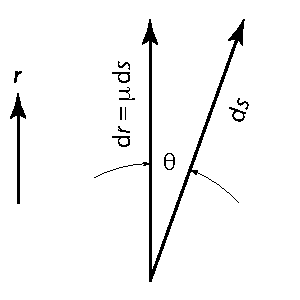
\includegraphics[width=\linewidth]{dr-ds-relation}
\caption[Coordinates for radiative transport equation]{\label{f.dr-ds-relation} Schematic of the coordinate system used for solving the radiative transport equation.}
\end{marginfigure}
We can now examine how heat transport works in the deep interior of a star. First, we need to establish our coordinate system. In equation~(\ref{e.transfer-equation}), the coordinate $s$ is distance along a ray; but it is more convenient to use coordinates that are tied to the star. We therefore use radial distance $r$ as a coordinate, and measure the optical depth along it: $\dif\tau_{\nu} = \rho\kappa_{\nu}\,\dif r$. 
Since $\dif r = \mu\,\dif s$, where $\mu=\cos\theta$ is the cosine between $\dif s$ and $\dif r$ (Fig.~\ref{f.dr-ds-relation}), the equation of transfer becomes
\begin{equation}
\mu\DD{I_{\nu}}{r} = -\rho\kappa_{\nu}\left(I_{\nu} - S_{\nu}\right).
\end{equation}

\newthought{Let's examine the typical scales of terms in the radiative transfer equation, for conditions in the deep solar interior.} We'll start by indicating some expected scales for eq.~(\ref{e.transfer-equation}):
\[
\underbrace{\mu\DD{I_{\nu}}{r}}_{\sim I_{\nu}/\Rsun} = -\underbrace{\rho\kappa_{\nu} I_{\nu}}_{\sim I_{\nu}/\ell}  +\rho\kappa_{\nu} S_{\nu}.
\]
If we are far from the surface of the star, then we should expect the intensity to change over lengthscales comparable to $\Rsun$. Of course, it won't be exactly this, but---as we'll show---the exact value doesn't matter so long as $|\dif I_{\nu}/\dif r|$ is in the ballpark of $I_{\nu}/\Rsun$. Notice the enormous disparity in scales:
\[
	\frac{|\dif I_{\nu}/\dif r|}{\rho\kappa_{\nu}I_{\nu}} \sim \frac{\ell}{\Rsun}.
\]
The left-hand side of eq.~(\ref{e.transfer-equation}) is smaller than the terms on the right by the ratio of the mean free path to the solar radius. This implies that conditions in the deep solar interior are nearly homogeneous. They are also isotropic, so that $I_{\nu} = J_{\nu}$. We expect that collisions are fast enough so that the matter is in thermal equilibrium and $j_{\nu} = \kapabs B_{\nu}$. We also know from exercise~\ref{ex.intensity-at-large-depth} that $I_{\nu} \to j_{\nu}/\kapabs = B_{\nu}$. From eq.~(\ref{e.simple-transfer}) it follows that $S_{\nu}= B_{\nu}$ as well.

We can't have $I_{\nu} = B_{\nu}$ exactly, however, since in that case there is no net flux! We'll therefore treat the intensity as being thermal plus a perturbation:
\[ I_{\nu} = B_{\nu} + I_{\nu}^{(1)}, \]
where the superscript ``(1)'' indicates that this is a small correction. Inserting this expansion into eq.~(\ref{e.transfer-equation}) and keeping only the lowest-order terms on each side gives
\begin{equation}\label{e.perturbation-radiative-transfer}
I_{\nu}^{(1)} = -\mu\DD{B_{\nu}}{\tau_{\nu}}.
\end{equation}
$B_{\nu}$ is a function of the temperature $T$, so $\dif B_{\nu}/\dif\tau_{\nu} = \dif B_{\nu}/\dif T \cdot \dif T/\dif \tau_{\nu}$. To get the flux, multiply eq.~(\ref{e.perturbation-radiative-transfer}) by $\mu$ and integrate over angles (cf.\ eq.~[\ref{e.specific-flux}]):
\[ F_{\nu} = \int\mu I_{\nu}^{(1)}\,\dif\Omega = -\int \mu^{2}\DD{B_{\nu}}{T}\,\DD{T}{\tau_{\nu}}\,\dif \Omega = -\frac{4\pi}{3} \DD{B_{\nu}}{T}\,\DD{T}{\tau_{\nu}}. \]
Switching variables from $\tau_{\nu}$ back to $r$ gives
\begin{equation}\label{e.specific-radiative-transport}
	F_{\nu} = -\frac{4\pi}{3}\left[\frac{1}{\rho\kappa_{\nu}}\dd{B_{\nu}}{T}\right]\DD{T}{r}.
\end{equation}
The flux $F_{\nu}$ is therefore proportional to the temperature gradient $\dif T/\dif r$, and
the term in $\left[\cdot\right]$ controls which frequencies have the largest flux and are therefore most responsible for energy transport.

\begin{exercisebox}[Transport by frequency]
\label{ex.radiative-transfer}
Let's examine the term $\left[\cdot\right]$ in eq.~(\ref{e.specific-radiative-transport}) more closely. Fig.~\ref{f.planck} shows $B_{\nu}$ and $\dif B_{\nu}/\dif T$ (top panel) and a hypothetical $\kappa_{\nu}$ (middle). Sketch $F_{\nu}$ on the bottom panel.  For which frequencies is it maximum?
\end{exercisebox}

\begin{marginfigure}
\includegraphics[width=\linewidth]{radiative-transfer-exercise}
\caption{\label{f.planck} The specific flux for a hypothetical opacity}
\end{marginfigure}

To get the total flux, we integrate $F_{\nu}$ over all frequencies. 
\begin{eqnarray*}
	F = \int_{0}^{\infty}F_{\nu}\,\dif\nu &=& -\frac{4\pi}{3} \left[\int_{0}^{\infty} \frac{1}{\rho\kappa_{\nu}}\dd{B_{\nu}}{T}\right]\DD{T}{r}\\
	&\equiv& -\frac{4\pi}{3}\frac{1}{\rho\kappa_{\mathrm{R}}}\dd{}{T}\left[\int_{0}^{\infty}B_{\nu}\,\dif\nu\right]\DD{T}{r}.
\end{eqnarray*}
Here we've defined the \newterm{Rosseland mean} of the opacity:
\begin{equation}\label{e.rosseland-opacity}
	\frac{1}{\kappa_{\mathrm{R}}} = \left(\int_{0}^{\infty} \dd{B_{\nu}}{T}\,\dif\nu\right)^{-1}\int_{0}^{\infty} \frac{1}{\kappa_{\nu}}\dd{B_{\nu}}{T}\,\dif\nu.
\end{equation}
This is a weighted average of $\kappa_{\nu}^{-1}$ with weight $\partial B_{\nu}/\partial T$. Since (cf.\ eq.~[\ref{e.bolometric-thermal-flux}]) $\int B_{\nu}\,\dif\nu = \sigmaSB T^{4}/\pi = c a T^{4}/4\pi$, we can write the equation for the flux as
\begin{equation}
	F = -\frac{1}{3}\frac{c}{\rho\kappa_{\mathrm{R}}}\DD{}{r}aT^{4}.
\label{e.radiative-transfer}
\end{equation}
Equation (\ref{e.radiative-transfer}) is known as the equation for radiative diffusion, for reasons that will become apparent in the next section.

If we multiply the flux by the surface area of a shell in the star we obtain the luminosity $L = 4\pi r^{2} F$; we can therefore recast eq.~(\ref{e.radiative-transfer}) into an equation for the thermal gradient:
\begin{equation}
    \label{e.gradient-temperature}
    \DD{T}{r} = -\frac{3\rho\kappa_{R}}{4acT^3}\frac{L(r)}{4\pi r^2}.
\end{equation}

\begin{exercisebox}[Radiative transfer equation]
\label{ex.radiative-transfer-diffusion}
Let's dissect eq.~(\ref{e.radiative-transfer}) to see how it sets the luminosity.  
\begin{enumerate}
\item\label{p.F-L}
To keep the algebra simple, assume that $F$ is constant throughout the star and that $aT^{4}$ is linear in $r$---that is, $aT^{4} = aT_{c}^{4}(1-r/R)$.  Since $F$ is constant, you can express it in terms of the luminosity at the surface $L$.  Use this to transform eq.~(\ref{e.radiative-transfer}) into an expression for $L$ in terms of $R$ and $T_{c}$ (along with $\rho$, $\kappa_{\mathrm{R}}$, and $c$).

\item\label{p.L-tau}
Write the luminosity as $L = E_{\gamma}/\tau$, where $E_{\gamma}$ is the total radiative energy of the star, and $\tau$ some as-yet-undetermined \emph{diffusion timescale}.  Give an estimate of $E_{\gamma}$ in terms of the mean temperature $T$ and the radius $R$ of the star.

\item\label{p.tau}
Finally, assume that the photon mean free path $\ell = (\rho\kappa_{\mathrm{R}})^{-1}$ is constant.  Substitute the results from parts \ref{p.F-L} and \ref{p.L-tau} into equation~(\ref{e.radiative-transfer}).  After simplifying, you should end up with a simple expression for $\tau$ in terms of $c$, $R$, and $\ell$.  For Thomson scattering, what is $\tau$ (express in years)?
\end{enumerate}
\end{exercisebox}

\section{Diffusion}\label{s.diffusion}

In the presence of scattering or absorption, photons take short hops averaging one mean free path $\ell$ in length. Imagine a small cube with sides of length $\ell$ and filled with photons. The total radiant energy in the cube is $\Delta E$. In a time $\Delta t = \ell/c$, all of the photons will leave this cube. The total luminosity of the cube is thus $\Delta E/\Delta t = c\Delta E/\ell$. If everything is isotropic, then the flux out of any one face is $1/6$ of the luminosity, divided by the area of that face:
\[
	F = \frac{1}{6\ell^{2}}\frac{c\Delta E}{\ell} = \frac{1}{6}c U,
\]
where $U = E/\ell^{3}$ is the radiative energy density. 

Now place two of these cubes against one another, with their common face located at position $x$. The energy density of the two cubes need not be the same; the energy density of the left cube is $U(x-\ell)$ and of the right cube is $U(x+\ell)$ (see Fig.~\ref{f.diffusive-flux}). The net flux traveling in the $x$-direction through the common face is then
\[
	F = {\color{blue}\frac{1}{6} c U(x-\ell)} - {\color{red}\frac{1}{6} c U(x+\ell)} \approx -\frac{1}{3}c\ell \DDx{U}.
\]
This is an expression for a \newterm{diffusive flux}. Although we gave a heuristic explanation, the formula is in general true:
\begin{eqnarray}
\nonumber
(\textrm{flux of something}) &=& -\frac{1}{3}\times(\textrm{speed of carriers})\times(\textrm{MFP of carriers})\\
&&\times \grad(\textrm{density of something})
\label{e.diffusive-flux}
\end{eqnarray}
For radiation, the ``something'' is ``radiative energy'' and the carriers are photons.
\begin{marginfigure}[-12\baselineskip]
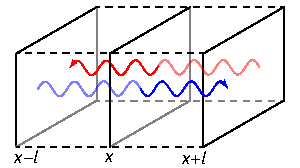
\includegraphics[width=\linewidth]{diffusive-flux}
\caption[Transport along a gradient]{\label{f.diffusive-flux} Illustration of net flux crossing a face between regions with slightly different energy densities.}
\end{marginfigure}

\begin{exercisebox}[Rosseland weighting]
Compare this diffusion equation,
\[
	F = -\frac{1}{3}c\ell\DD{U}{r},
\]
with eq.~(\ref{e.radiative-transfer}) and use eq.~(\ref{e.rosseland-opacity}) to write an expression for the \emph{average} mean free path  of a photon (the ``mean mean free path''?). Can you give a physical interpretation for the weighting function used in computing the average (cf.\ exercise \ref{ex.radiative-transfer})?
\end{exercisebox}

\begin{marginfigure}
\includegraphics[width=\linewidth]{random-walk-schematic}
\caption[Schematic of a random walk]{\label{f.random-walk-schematic}Schematic of a random walk of 50 steps.}
\end{marginfigure}
\newthought{For an alternate view on photon diffusion,} imagine a photon random-walking throughout the stellar interior.
The photon moves at speed $c$, but it can only go one mean free path $\ell$ before being absorbed or scattered, at which point it is sent off in a random direction. The path of the photon will therefore look something like that in Fig.~\ref{f.random-walk-schematic}.

We will just do our calculation for motion along a diameter, with the photon starting at the center. On each hop, the photon either goes left or right with equal probability.\marginnote{To keep things simple, we'll imagine that after absorption the atom immediately emits an identical photon in a random direction.} On average, the photon doesn't go anywhere; but after enough hops, there is some probability for the photon to reach the edge of the star and escape. Figure~\ref{f.random-walk} shows the distribution of positions for walks of length $n = 10, 30, 100, 300$ steps, with each step having length 1.0. Suppose the edge of the star is at $x=\pm 10$ (red dotted lines).  Although the average position is at $x=0$, for $n \gtrsim 100$ steps, there is a reasonable probability of the photon eventually escaping.
\begin{figure}[htbp]
\includegraphics[width=\linewidth]{random-walk}
\caption[Distribution of positions in a random walk]{\label{f.random-walk} Distribution of positions after $n$ steps in a random walk.}
\end{figure}

Recall that a random walk is described by a binomial distribution: after $n$ steps, the probability that $m$ of them were to the right is
\begin{equation}\label{e.binomial}
    \binom{n}{m}{p} = \frac{n!}{m!(n-m)!} p^{m}(1-p)^{n-m}.
\end{equation}
Here $p$ is the probability of any single step being to the right.
The mean and root variance of $m$ are
\begin{eqnarray}
	\mean{m} &=& np \label{e.mean-binomial} \\
	\left[\mean{\left(m-\mean{m}\right)^{2}}\right]^{1/2} &=& \left[np(1-p)\right]^{1/2}. \label{e.var-binomial}
\end{eqnarray}
In exercise \ref{ex.random-walk-diffusion}, you will use these quantities to estimate the diffusion timescale $\tau$.

\begin{exercisebox}[Radiative diffusion as a random walk]
\label{ex.random-walk-diffusion}
\begin{enumerate}
\item
Show from equation~(\ref{e.mean-binomial}) that the mean distance traveled by the photon after $n$ steps is $\langle d\rangle = \ell(2np-n)$, so for $p=1/2$, $\langle d\rangle = 0$.

\item\label{p.straight-line-steps}
If all the steps were in the same direction, how many steps would be needed to reach the edge, at a a distance $R$ from the center? Assume all steps have the same length $\ell$.

\item
We want the distribution of steps (cf.\ Fig.~\ref{f.random-walk}) to be wide enough to reach the edge. Set the root variance---a measure of the width of the probability distribution---equal to the number of steps found in part \ref{p.straight-line-steps} and use equation~(\ref{e.var-binomial}),
	\[
		\left[\mean{\left(m-\mean{m}\right)^{2}}\right]^{1/2} = 
			\left[n_{\mathrm{edge}}p(1-p)\right]^{1/2},
	\]
	to find $n_{\mathrm{edge}}$ in terms of $R$ and $\ell$.

\item
What is the \emph{total} distance traveled by the photon after $n_{\mathrm{edge}}$ steps? If the photon traveled at speed $c$, how long did it take? Compare your answer with that for part~\ref{p.tau} of exercise~\ref{ex.radiative-transfer-diffusion}.

\end{enumerate}
\end{exercisebox}

\section{The photosphere}

We are now ready to investigate heat transport near the star's edge, where the optical depth $\tau_{\nu} \lesssim 1$ and photons begin to freely escape. Near the edge, we cannot use the approximation of radiative diffusion, because conditions are changing over distances of order one mean free path. We therefore return to equation~(\ref{e.transfer-equation}) for radiative transport:
\[
	\DD{I_{\nu}}{s} = -\rho\left(\kapabs + \kapscat\right) I_{\nu} + \rho j_{\nu} + \rho\kapscat J_{\nu}.
\]
This is difficult to solve: for some frequencies, the atmosphere is nearly transparent, while for other frequencies it is quite opaque. Rather than develop the numerical machinery to solve this equation, we shall make a few simplifying assumptions (indicated by \colorbox{yellow}{\textbf{highlighted bold text}} in the margins) to obtain an approximate solution for the temperature of the stellar atmosphere.

\marginnote[\baselineskip]{\colorbox{yellow}{\textbf{Opacities are gray}}}First, we assume that the opacity is gray---that is, independent of frequency. Although unphysical, the solutions for temperature and pressure near the stellar photosphere will still have the correct qualitative behavior. Because the opacity is gray, we shall drop the ``$\nu$'' subscript in $\kappa$ and $\tau$.

\begin{exercisebox}[Gray emissivity?]
Does matter with a gray opacity in thermal equilibrium also have a gray emissivity $j_{\nu}=j$?
\end{exercisebox}

We next define a coordinate system. Since we are in a thin layer near the edge of the star, we will adopt planar coordinates, with $z$ being the altitude above some point. We'll pick $z=0$ to be a point deep enough in the star that $I_{\nu}\approx B_{\nu}$. Then we define the optical depth as
\begin{equation}\label{e.optical-depth-planar}
	\tau(z) = \int_{z}^{\infty} \rho\left(\kappa^{\mathrm{abs}}+\kappa^{\mathrm{sca}}\right)\,\dif z ;
\end{equation}
differentiating this expression gives
\[
	\DD{\tau}{z} = -\rho\left(\kappa^{\mathrm{abs}}+\kappa^{\mathrm{sca}}\right) \equiv -\rho\kappa.
\]
Note the ``$-$'': in these coordinates, as $z$ gets larger, $\tau$ gets smaller. Alternatively, you can view $\tau$ as being the optical depth for a photon traveling \emph{into} the star.

Using eq.~(\ref{e.optical-depth-planar}), we then rewrite the equation of hydrostatic balance (\ref{e.hydrostatic-equilibrium-g}) as
\begin{eqnarray}
	-\rho g = \DD{P}{z} &=& \DD{P}{\tau}\DD{\tau}{z} = -\rho\kappa\DD{P}{\tau},\nonumber\\
	\DD{P}{\tau} &=& \frac{g}{\kappa}.
\label{e.P-tau}
\end{eqnarray}
Since we are in a thin layer, we can take the gravitational acceleration $g$ to be approximately constant. By integrating hydrostatic equilibrium from where $\tau = 0, P = 0$ to where $\tau = 1$, we obtain an approximate value of the photospheric pressure,
\[
	P_{\mathrm{ph}} = \int_{0}^{P_{\mathrm{ph}}}\,\dif P = \int_{0}^{1}\frac{g}{\kappa}\,\dif\tau \approx \frac{g}{\kappa}.
\]
\begin{quote}
\emph{The surface gravity sets the pressure at the \textbf{photosphere}, the location where the optical depth is of order unity and where photons can escape from the star.}
\end{quote}

\begin{exercisebox}[Photospheric pressure]
Suppose you observe a star that has a 10\% larger mass and 10\% larger radius than the sun. All else being equal, how does the pressure at the photosphere of this star compare to that of the sun?
\end{exercisebox}

For our second approximation, we assume that the matter is in \newterm{local thermal equilibrium} (LTE). This means there is a well-defined temperature at each depth. Furthermore, the emissivity is related to the absorption opacity,
\marginnote[-2\baselineskip]{\colorbox{yellow}{\textbf{Atmosphere is in steady-state LTE}}} 
\[
	j_{\nu} = \kappa^{\mathrm{abs}}B_{\nu}.
\]
Note that this does \emph{not} imply the radiation field is actually Planckian.

We then take the radiative transfer equation (\ref{e.transfer-equation}) and substitute our definition of optical depth (eq.~[\ref{e.optical-depth-planar}]) to obtain
\begin{equation}\label{e.transfer-gray}
	\mu\DD{I_{\nu}}{\tau} = I_{\nu} - S_{\nu}.
\end{equation}
Here
\[
	S_{\nu} = \frac{j_{\nu} + \kappa^{\mathrm{sca}} J_{\nu}}{\kappa}
	= \frac{\kappa^{\mathrm{abs}} B_{\nu} + \kappa^{\mathrm{sca}} J_{\nu}}{\kappa}.
\]
If, in addition, the matter is in steady-state, then the rate at which energy is absorbed from the radiation field, $\int\kappa^{\mathrm{abs}}I_{\nu}\,\dif\nu\,\dif\Omega$, must equal the rate at which energy is emitted, $\int j_{\nu}\,\dif\nu\,\dif\Omega$:
\begin{eqnarray*}
	\int \left(j_{\nu} - \kappa^{\mathrm{abs}}I_{\nu}\right)\,\dif\nu\,\dif\Omega
	&=& \kappa^{\mathrm{abs}}\int\left(B_{\nu} - I_{\nu}\right)\,\dif\nu\,\dif\Omega\\
	&=& 4\pi\kappa^{\mathrm{abs}}\int\left(B_{\nu} - J_{\nu}\right)\,\dif\nu 
	= 0.
\end{eqnarray*}
In this expression we use the LTE expression for $j_{\nu}$ and we pull $\kappa^{\mathrm{abs}}$ from the integral because it is independent of frequency.

Since $J = \int J_{\nu}\,\dif\nu = \int B_{\nu}\,\dif\nu = B$, it follows that $S = \int S_{\nu}\,\dif\nu = B$ as well.
\begin{quote}
\emph{For a gray atmosphere in steady-state, local thermal equilibrium, the integrated source function and mean intensity equal the Planck value:}
\[ S(\tau) = J(\tau) = B(\tau), \]
\end{quote}
Note that this does \emph{not} imply that $I_{\nu}=B_{\nu}$ or $J_{\nu}=B_{\nu}$: it only means their frequency-integrated averages are equal.

If we integrate eq.~(\ref{e.transfer-gray}) over all angles,
\begin{eqnarray*}
	\int\mu\DD{I_{\nu}}{\tau}\,\dif\Omega &=& \int I_{\nu}\,\dif\nu -\int S_{\nu}\,\dif\Omega\\
	\DD{F_{\nu}}{\tau} &=& 4\pi \left(J_{\nu} - S_{\nu}\right),
\end{eqnarray*}
and then integrate over all frequencies and use the steady-state, LTE relation,
\[ \DD{F}{\tau} = \DD{}{\tau}\int F_{\nu}\,\dif\nu = 4\pi\int \left(J_{\nu} - S_{\nu}\right)\,\dif\nu = 0.\]
We thus have the remarkable result:
\begin{quote}
\emph{For a steady-state gray atmosphere in local thermal equilibrium, the total flux $F = \int F_{\nu}\,\dif\nu$ is constant.}
\end{quote}
That is, the atmosphere does not add to, or detract from, the radiation flowing through it.

We still have the problem that eq.~(\ref{e.transfer-gray}) includes both the derivative and integral of $I_{\nu}$. To get around this, we expand $I_{\nu}$ in Legendre polynomials\sidenote{see Box~\ref{sb.intensity-decomposition}},
\[
	I_{\nu}(\tau,\mu) = I_{\nu,0}(\tau)\Pl{0}(\mu) + I_{\nu,1}(\tau)\Pl{1}(\mu) + I_{\nu,2}(\tau)\Pl{2}(\mu) + \ldots
\]
and only retain the first two terms, $\Pl{0}(\mu) = 1, \Pl{1} = \mu$. That is, we assume $I_{\nu}$ is \emph{linear} in $\mu$: $I_{\nu} = I_{\nu,0}(\tau) + I_{\nu,1}(\tau)\mu$. 
\marginnote{\colorbox{yellow}{\textbf{Intensity is linear in $\mu$}}}

In terms of this expansion, the angle-averaged specific intensity is
\[
	J_{\nu}(\tau) = \frac{1}{4\pi}\int I_{\nu}\,\dif\mu\,\dif\phi = I_{\nu,0}(\tau),
\]
and hence the specific energy density is $U_{\nu} = 4\pi/c\cdot J_{\nu} = 4\pi/c\cdot I_{\nu,0}$. The specific flux is
\[
	F_{\nu}(\tau) = \int \mu I_{\nu}\,\dif\mu\,\dif\phi = \frac{4\pi}{3} I_{\nu,1}(\tau).
\]
We can therefore use these relations for $I_{\nu,0}$ and $I_{\nu,1}$ to express the intensity as
\begin{equation}
\label{e.intensity-expanded}
I_{\nu}(\tau) = \frac{c}{4\pi}U_{\nu}(\tau) + \frac{3\mu}{4\pi} F_{\nu}(\tau).
\end{equation}

\begin{sidebar}[Expansion in Legendre polynomials]
\label{sb.intensity-decomposition}
You may recall from electrostatics that we can decompose the field from a set of charges into a sum of moments: dipole, quadrupole, and so on. The basis functions for this expansion are the Legendre polynomials $\Pl{n}(\cos\theta)$, defined via
\[
	\frac{1}{\sqrt{1 - 2\mu z + z^{2}}} \equiv \sum_{n=0}^{\infty}\Pl{n}(\mu)z^{n},
\]
for $-1<\mu<1,\;|z| < 1$. The first four polynomials are
\begin{eqnarray*}
	\Pl{0}(\mu) = 1 &\quad& \Pl{2}(\mu) = \frac{1}{2}(3\mu^{2}-1)\\
	\Pl{1}(\mu) = \mu &\quad& \Pl{3}(\mu) = \frac{1}{2}(5\mu^{3}-3\mu),
\end{eqnarray*}
and the first eight Legendre polynomials are plotted below.

\includegraphics{legendre}

\noindent As $n$ increases, the angular variations become finer.

The Legendre polynomials are \emph{orthogonal} in the following sense:
\begin{equation}\label{e.orthogonal}
\int_{-1}^{1}\Pl{n}(\mu)\Pl{m}(\mu)\dif \mu = \left\{
\begin{array}{lr}
	0 &  m\neq n\\
	\frac{2}{2n+1} & m=n
\end{array}\right..
\end{equation}
As a result of this orthogonality, we can decompose the radiative intensity into multipoles:
\begin{equation}\label{e.decomposition}
	I = \sum_{n=0}^{\infty} I_{n} \Pl{n}(\mu).
\end{equation}

\begin{exercisebox}[Odd-even powers of $\mu$]
\label{e.symmetry-powers-mu}
Use eq.~(\ref{e.orthogonal}) to show that $(4\pi)^{-1}\int I\,\dif\Omega = I_{0}$ and $\int \mu I\,\dif\Omega = (4\pi/3)I_{1}$, for $I = I_{0} + I_{1}\mu$.
\end{exercisebox}

\end{sidebar}

Since the flux in the atmosphere is constant, it must be equal to its value far from the star where $\tau\to0$: $F(\tau=0) = \sigmaSB\,\Teff^{4}$. We can therefore integrate eq.~(\ref{e.intensity-expanded}) over frequency and substitute for $F$:
\begin{equation}
\label{e.Inu-expansion}
	I(\mu,\tau) = \frac{c}{4\pi} U(\tau) + \frac{3\mu}{4\pi}\sigmaSB\Teff^{4}.
\end{equation}
To solve for $U(\tau)$, integrate eq.~(\ref{e.transfer-gray}) over frequency,
$\mu\,\dif I/\dif\tau = I-S$, substitute for $I$ on the left-hand side using eq.~(\ref{e.Inu-expansion}), then multiply by $\mu$ and integrate over all angles:
\begin{eqnarray}
	\DD{}{\tau}\int\mu^{2}I\,\dif\Omega &=& \int\mu I\,\dif\Omega
		- \int \mu S\,\dif\Omega\nonumber\\
	\frac{c}{4\pi}\DD{}{\tau} \int \mu^{2}U\,\dif\Omega 
		+ \frac{3}{4\pi}\sigmaSB\Teff^{4}\int\mu^{3}\,\dif\Omega &=& F - \int \mu S\,\dif\Omega\nonumber\\
	\frac{c}{3}\DD{U}{\tau} &=& F = \sigmaSB\Teff^{4}
\label{e.ODE-U}
\end{eqnarray}
The integrals over $\mu^{3}$ and $\mu S$ vanish because $S$ is independent of angle and $\int_{-1}^{1} \mu\,\dif\mu = \int_{-1}^{1}\mu^{3}\,\dif\mu = 0$. Also, $U$ is independent of $\mu$, and $\int\mu^{2}\,\dif\Omega = \int_{0}^{2\pi}\int_{-1}^{1}\mu^{2}\,\dif\mu\,\dif\phi = (4\pi/3)$.

Equation~(\ref{e.ODE-U}) is a first-order ODE, which upon integration yields
\begin{equation}\label{e.energy-density-Eddington}
	U(\tau) = \frac{3}{c}F(\tau + \tau_{0}) = \frac{3}{c}\sigmaSB\Teff^{4} (\tau+\tau_{0}),
\end{equation}
where $\tau_{0}$ is an integration constant. Substituting this back into the expression for the intensity, eq.~(\ref{e.Inu-expansion}), gives
\[
	I(\mu,\tau) = \frac{3}{4\pi}\sigmaSB\Teff^{4}\left(\tau + \tau_{0} + \mu\right).
\]
To fix the integration constant $\tau_{0}$, evaluate this expression at $\tau=0$. Far outside the star, all of the radiation must be outward-bound. Hence if we integrate $\mu I(\mu,\tau=0)$ over $0\le\mu\le 1$, we should recover the flux:
\[
	\sigmaSB\Teff^{4} = \int_{0}^{2\pi}\int_{0}^{1} \mu I(\mu,\tau=0)\,\dif\mu\,\dif\phi
	= \frac{3}{4}\sigmaSB\Teff^{4}\left(\tau_{0} + \frac{2}{3}\right),
\]
which fixes $\tau_{0} = 2/3$.

We are almost finished! To recap, we now have the expressions for the intensity, flux, and radiative energy density under the assumption of a gray atmosphere in steady-state, local thermal equilibrium and under the approximation of the intensity being linear in $\mu$:
\begin{eqnarray*}
I &=& \frac{3}{4\pi}\sigmaSB\Teff^{4}\left(\tau + \mu + \frac{2}{3}\right)\\
F &=& \sigmaSB\Teff^{4}\\
U &=& \frac{3}{c}\sigmaSB\Teff^{4}\left(\tau + \frac{2}{3}\right).
\end{eqnarray*}
To finish this, we note that in the atmosphere $J = B$ since we are in steady-state local thermal equilibrium. The radiative energy density can thus be written as $U(\tau) = (4\pi/c) J(\tau) = (4\pi/c)B(\tau) = (4\sigmaSB/c )T^{4}(\tau)$. Substituting this into eq.~(\ref{e.energy-density-Eddington}) gives us an expression for the temperature in terms of optical depth,
\begin{equation}\label{e.T-tau}
T^{4}(\tau) = \frac{3}{4}\Teff^{4}\left(\tau + \frac{2}{3}\right).
\end{equation}
This equation, along with eq.~(\ref{e.P-tau}), determines the structure of the stellar atmosphere.

\begin{sidebar}[Decomposition of intensity into moments]
\label{sb.intensity-moments}
Our integration of the radiative-transfer equation~(\ref{e.transfer-gray}) is known as taking a \newterm{moment} of the equation. A moment is simply a weighted average, where the weight is a power of $\mu$. For example, to take the zeroth-order moment of the radiative intensity, we multiply $I_{\nu}$ by $\mu^{0}=1$, integrate over all angles, and divide by $4\pi$:
\[
	J_{\nu} = \frac{1}{4\pi}\int_{0}^{2\pi}\int_{-1}^{1} I_{\nu}\,\dif\mu\,\dif\phi.
\]
To take the first-order moment $H_{\nu}$, we use a weight $\mu^{1}$:
\[
	H_{\nu} = \frac{1}{4\pi}\int_{0}^{2\pi}\int_{-1}^{1}\mu I_{\nu}\,\dif\mu\,\dif\phi.
\]
To take the second-order moment $K_{\nu}$, we use a weight $\mu^{2}$:
\[
	K_{\nu} = \frac{1}{4\pi}\int_{0}^{2\pi}\int_{-1}^{1}\mu^{2} I_{\nu}\,\dif\mu\,\dif\phi.
\]
The first three moments have physically interpretable meanings: the specific radiative energy density, flux, and pressure are $U_{\nu} = (4\pi/c)J_{\nu}$, $F_{\nu} = 4\pi H_{\nu}$, and $P_{\nu} = (4\pi/c) K_{\nu}$, respectively.

By taking moments of the radiative-transfer equation~(\ref{e.transfer-gray}), we reduce the complicated integro-differential equation into a simpler ordinary differential equation. This comes at a cost, however; because the left-hand side contains $\mu\dif/\dif\tau$, the left hand side will have a higher-order moment than the right-hand side. By multiplying eq.~(\ref{e.transfer-gray}) by successively higher powers of $\mu$ and integrating, we generate an infinite series of ODE's for successively higher moments of $I_{\nu}$. The trick to this procedure is to adopt a \newterm{closure relation} that truncates this series. The classic scheme, attributed to Eddington, is to take $K = J/3$. The Eddington closure scheme is equivalent to expanding the radiative intensity to terms linear in $\mu$.

\begin{exercisebox}[The Eddington closure scheme]
Show that if we approximate the intensity as $I_{\nu}(\mu,\tau) = I_{\nu,0}(\tau) + \mu I_{\nu,1}(\tau)$ (cf.\ eq.~[\ref{e.intensity-expanded}]), then $K_{\nu} = J_{\nu}/3$ identically.
\end{exercisebox}
\end{sidebar}

\begin{exercisebox}[Anisotropy of the intensity]
Deep in the star, we expect the radiation to be nearly isotropic, while it becomes outward-bound as $\tau\to 0$. Let's investigate this. We'll measure the anisotropy of the radiation field using the first two moments of the intensity (Box~\ref{sb.intensity-moments}).
\begin{enumerate}
\item
Demonstrate that $H_{\nu}/J_{\nu} = 0$ if the radiation is isotropic.

\item
Next, suppose the radiation is completely anisotropic: all the photons are headed in a narrow cone about the direction $\mu = 1$. To make this precise, let
\[
	I_{\nu}(\mu) = \left\{
		\begin{array}{lr}
			I_{\nu,0} & 1-\varepsilon \le \mu \le 1,\\
			0 & \textrm{otherwise,}
		\end{array}
	\right.
\]
where $I_{\nu,0}$ is a constant. Show that $H_{\nu}/J_{\nu} \to 1$ as $\varepsilon\to 0$.

\item
Now compute $H(\tau)/J(\tau)$ for our gray atmosphere.What is the degree of anisotropy at $\tau = 0$? at $\tau=2/3$? at $\tau = 10$?
\end{enumerate}
\end{exercisebox}


